\documentclass[conf]{new-aiaa}
%\documentclass[journal]{new-aiaa} for journal papers
\usepackage[utf8]{inputenc}

\usepackage{graphicx}
\usepackage{amsmath}
\usepackage[version=4]{mhchem}
\usepackage{siunitx}
\usepackage{longtable,tabularx}
\usepackage[table, dvipsnames]{xcolor}
\usepackage{color,soul}
\setlength\LTleft{0pt} 

\title{Modeling Stanford Football Betting as an MDP with Q-Learning}

\author{Sean Auer and Zain Jamal}
\affil{Stanford University, Stanford, CA, 94305, United States of America}


\begin{document}

\maketitle

\begin{abstract}
Filler words to hold the space for now. This section will be the abstract. Don't forget about it whoever ends up writing it. Please and thank you very much. Very nice abstract.
\end{abstract}

\section{Nomenclature}

{\renewcommand\arraystretch{1.0}
\noindent\begin{longtable*}{@{}l @{\quad=\quad} l@{}}
$B$ &  Bet amount \\
$E$ &  Elo \\
$D$ &  Elo differential scaling parameter\\
$o$ &  Stanford moneyline odds \\

\end{longtable*}}

\section{Introduction}
Introduce sports data environment, how betting works. Lay out objective of project, problem statement with assumptions, and what the reader should expect. Make sure to mention we are simulating the 2023 season. We can just cite our reason as the season wasn't over when we started this, but it's really because the results are worse for 2024.

\section{Data Formatting}

Data for this project was obtained from \textit{collegefootballdata.com} (from here on out referred to as \textit{cfd.com}), a free-to-use, third party website tracking all NCAA football games dating back to 1869 \hl{(https://collegefootballdata.com/)}. With recent advancements in sports metrics, \textit{cfd.com} has added a plethora of datasets pertaining to different topics. Four different datasets from \textit{cfd.com} were deemed important to this project and are listed below.
\begin{enumerate}
    \item Betting lines: This dataset contained a number of betting odds for Stanford's football games. The moneyline odds from this dataset were used to calculate the reward for a game week should an agent bet on Stanford to win. The betting data had entries prior to 2021, so the scope of the data in this project is constrained to the 2021, 2022, and 2023 seasons.
    \item Game statistics: This dataset contained the scores of each game week, the pregame Elo $(E)$ rating of both teams, which is a metric used to measure general team strength, and the excitement index, a measurement of how exciting a game is based on shifts in win probability.
    \item Team statistics: This dataset provided basic statistics of Stanford football for each week, such as touchdowns, passing yards, rushing yards, interceptions, etc. The algorithm can run through these statistics to detect patterns leading to wins, and therefore an optimal betting strategy.
    \item Advanced metrics: This dataset contained a number of calculated metrics such as predicted points added (PPA), explosiveness, success rates, and possession time. These metrics are often used by sports analytics professionals to predict game outcomes. Similar to the team statistics, this project uses the advanced metrics to define the states and develop a decision-making policy accordingly.
\end{enumerate}
In order to iterate through the football season sequentially, the data had to be combined and arranged by game week, which not all datasets were. The data was reformatted so every betting line, score, statistic, and metric belonged to one row representing a single game. Some games against smaller schools did not have available betting data, such as the 2023 game against Sacramento State or the 2022 game against Colgate, so all associated data was omitted. The end result was two datasets to provide the foundation of the algorithms. The first was an 11 x 124 (games x pertinent data) matrix representing the 2023 season to be simulated as if it was current day. The second was a 24 x 124 matrix representing the 2021 and 2022 seasons to be used for training the learning algorithm. A majority of, but not all, 124 data entries were used to define the state, as is explained in the following section. 

For reference to the reader, the Stanford football team finished with a record of three wins and eight losses during the 2023 season, which presents three opportunities for a successful bet yielding a profit and eight opportunities for an unsuccessful bet resulting in a loss. This information would not be available to the betting agent, as they can only access information from past seasons or games that have already been played in the current season. 


\section{Decision-Making Algorithm}



\subsection{MDP Formulation}
Lay out states, actions, rewards, transitions and any built equations. Use fancy letters for arbitrary parameters where possible. States are the only difference between the two algorithms, so maybe explain those in the corresponding next sections. Define bet amount in reward function.

\subsection{Deterministic Policy}

\begin{equation}
\label{win prob}
P(win) = \frac{1}{1 + 10^{-\frac{\Delta E}{D}}}
\end{equation}

where $\Delta E$ is the Stanford Elo subtracted by the Opponent Elo, a variable defined the measure the difference in skill between the opposing teams. $D$ is a user defined parameter used to scale how much the differences in $E$ impact the probability of Stanford to win. Through trial and error, $D=400$ yielded the best results. The win probability was then used to calculate the expected value using the moneyline odds, $o$, as shown below. 
\begin{equation}
\$U_E = 
\begin{cases} 
\$B \times \left( P(win) \times \frac{o}{100} - (1 - P(win)) \right) & \text{if } o > 0 \\
\$B \times \left( P(win) \times \frac{100}{|o|} - (1 - P(win)) \right) & \text{if } o \leq 0
\end{cases}
\end{equation}

The expected value of the bet was compared to a user-defined threshold value of 5. If the expected value was above the threshold, the agent took the bet. 




\subsection{Q-Learning}
Talk about how Q-learning is implemented (or whatever method ends up being used). Reference code in github. Could use appendix to define whole state space

\section{Results \& Discussion}


\begin{figure}[h]
    \centering
    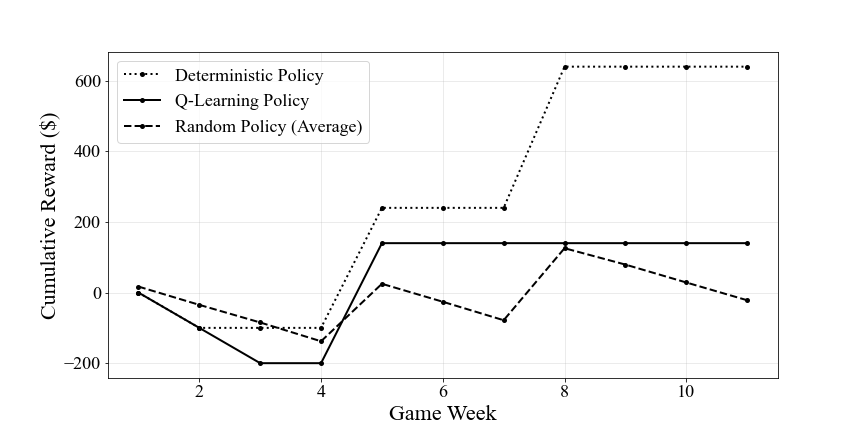
\includegraphics[scale=.5]{Reward-Time.png}
    \caption{Caption}
    \label{fig:enter-label}
\end{figure}

\begin{figure}[h]
    \centering
    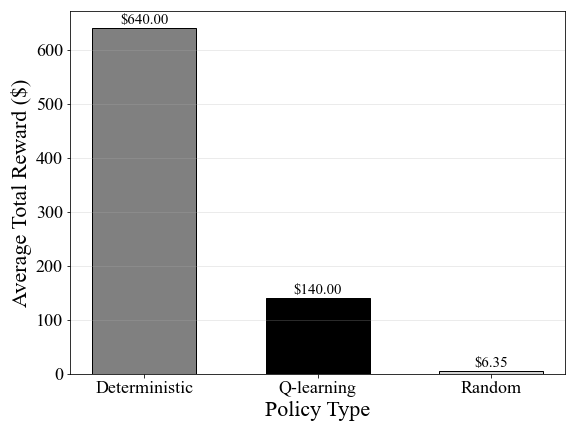
\includegraphics[scale=.5]{AvgReward.png}
    \caption{Caption}
    \label{fig:enter-label}
\end{figure}

\begin{table}[h]
\caption{\label{tab:table1} Transitions selected for thermometry}
\centering
\begin{tabular}{lcccccc}
\hline
Policy Algorithm& Win Predictions & Loss Predictions& Success Over Random Policy\\\hline
Deterministic & 67.7\%& 87.5\%& 98.2\%\\
Q-Learning& 33.3\%& 75.0\%& 70.1\%\\
\hline
\end{tabular}
\end{table}

\section{Conclusion}
Resummarize the whole paper, give some insights on why the algorithm did or did not perform. Deterministic probably would have to be tuned from season to season but isn't thrown off by previous season's data. Q-learning had worse results probably because the team changes. Still good results. Would someone use the model in real life? Discuss possible improvements and link github.

\section{Table of Contributions}


\begin{center}
\begin{tabular}{ |c|c| } 
\hline
\rowcolor{lightgray}
\textbf{Zain}& \textbf{Sean}\\
\hline
This is Zain's contribution & This is Sean's contribution\\ 
\hline
\end{tabular}
\end{center}


\section*{Appendix}

Can maybe put data matrices used

\bibliography{sample}

\end{document}
